% This must be in the first 5 lines to tell arXiv to use pdfLaTeX, which is strongly recommended.
\pdfoutput=1
% In particular, the hyperref package requires pdfLaTeX in order to break URLs across lines.

\documentclass[11pt]{article}

% Remove the "review" option to generate the final version.
\usepackage{EACL2023}

% Standard package includes
\usepackage{times}
\usepackage{latexsym}
\usepackage{graphicx}

% For proper rendering and hyphenation of words containing Latin characters (including in bib files)
\usepackage[T1]{fontenc}
% For Vietnamese characters
% \usepackage[T5]{fontenc}
% See https://www.latex-project.org/help/documentation/encguide.pdf for other character sets

% This assumes your files are encoded as UTF8
\usepackage[utf8]{inputenc}

% This is not strictly necessary, and may be commented out.
% However, it will improve the layout of the manuscript,
% and will typically save some space.
\usepackage{microtype}

% This is also not strictly necessary, and may be commented out.
% However, it will improve the aesthetics of text in
% the typewriter font.
\usepackage{inconsolata}
\usepackage{float}

% If the title and author information does not fit in the area allocated, uncomment the following
%
%\setlength\titlebox{<dim>}
%
% and set <dim> to something 5cm or larger.

\title{Language Identification from Audio}

% Author information can be set in various styles:
% For several authors from the same institution:
% \author{Author 1 \and ... \and Author n \\
%         Address line \\ ... \\ Address line}
% if the names do not fit well on one line use
%         Author 1 \\ {\bf Author 2} \\ ... \\ {\bf Author n} \\
% For authors from different institutions:
% \author{Author 1 \\ Address line \\  ... \\ Address line
%         \And  ... \And
%         Author n \\ Address line \\ ... \\ Address line}
% To start a seperate ``row'' of authors use \AND, as in
% \author{Author 1 \\ Address line \\  ... \\ Address line
%         \AND
%         Author 2 \\ Address line \\ ... \\ Address line \And
%         Author 3 \\ Address line \\ ... \\ Address line}

\author{
  Samruddhi M. Kulkarni \\
  Universität des Saarlandes \\
  \texttt{saku00003} \\\And
  Emadeldin M. Ibrahim \\
  Universität des Saarlandes \\
  \texttt{emmo00008} \\\And
  Fouzia Nasreen \\
  Universität des Saarlandes \\
  \texttt{fona00001} \\}
  
\begin{document}
\maketitle


\begin{abstract}
This project explores spoken language identification (SLID) under limited speaker diversity, where models have a likelihood of learning speaker specific acoustic patterns rather than language level characteristics. A baseline system using MMS-300m with 31.96\% validation accuracy was achieved and 35.67\% with hyperparameter tuning.  Pivoting to multil ingual mHuBERT-147 model and freezing the CNN feature encoder further significantly improved performance to 59.3\%. To address speaker bias, dynamic audio augmentation was applied during training, including speed perturbation, pitch shifting, and Gaussian noise, which prevented shortcut learning through speaker specific cues. Confusion matrix and t-SNE analysis further confirmed that learned representations align more closely with language boundaries rather than speaker identity. Our results suggest that speaker bias in this setting is rather concerning which only augmentation cannot completely resolve, and may require more sophisticated approaches such as adversarial training via Domain Adversarial Neural Networks (DANN) or speaker embedding subtraction using pretrained speaker verification models.
\end{abstract}

\section{Introduction}

Spoken Language Identification involves recognizing the language directly from audio without depending on transcripts or text. Latest developments in self-supervised learning have driven models like wave2vec 2.0 \cite{baevski2020wav2vec20frameworkselfsupervised} and HuBERT \cite{hsu2021hubertselfsupervisedspeechrepresentation} to the forefront of speech processing, as they have been shown to capture rich acoustic features from large unlabeled speech.
However, a less explored challenge arises when training data includes very few speakers per language. In such a case, model can learn to recognize voices rather than languages.This is a form of shortcut learning \cite{Geirhos_2020} and it quietly undermines how well the model generalizes to new speakers.
In this work, the dataset contains five speakers per 22 official Indian languages, making this problem especially relevant. This study pursues three goals: establishing strong baseline system, mitigate speaker bias through data centric and regularization based strategies, and analyzing learned representations to verify whether model encodes language or speaker identity.

\section{Methods}

\subsection{Model Architecture}
SLID system is based on pretrained self-supervised speech encoders followed by classification layers. These models learn general acoustic patterns from large speech dataset and can be adapted to downstream tasks with limited labeled data.
\\ Several pretrained encoders like mms-330m \cite{pratap2023scalingspeechtechnology1000}, wave2vec and mHuBERT were explored. Among these , the multilingual mHuBERT-147 was selected \citep{boito2024mhubert147compactmultilingualhubert} due to its ability to capture cross-lingual acoustic patterns that are instrumental for multilingual language identification.

\subsection{Encoder Freezing Strategy}
Early experiments showed unstable learning and validation accuracy close  to random guessing, suggesting the model was overfitting to speaker-specific  patterns rather than learning language features. During fine-tuning, the convolutional feature encoder was frozen to prevent overfitting to low-level speaker-specific patterns. Prior work has shown that lower layers of 
self-supervised speech models capture general acoustic features learned  during large-scale pre-training \cite{pasad2021layerwise}, while freezing  lower layers during fine-tuning is an established strategy for preserving pretrained representations \cite{howard2018universallanguagemodelfinetuning}. This allows the higher transformer layers to adapt to the language identification task without  corrupting low-level acoustic features.
\begin{table*}[t]
\centering
\small
\begin{tabular}{llc}
\hline
\textbf{Model} & \textbf{Configuration} & \textbf{Val. Acc.} \\
\hline
MMS-300m      & Baseline, lr=1e-5, 5s                              & 35.7\% \\
Wav2Vec2      & lr=1e-5, 5s                                        & 18.1\% \\
mHuBERT-147   & lr=1e-5, 5s                                        & $\sim$9\% \\
mHuBERT-147   & lr=5e-6, 10 epochs                                 & $\sim$12\% \\
mHuBERT-147      & Frozen encoder, lr=1e-5, 10s                            & 59.3\% \\
mHuBERT-147   & Frozen encoder, 10s, no aug.                   & $\sim$62\% \\
\textbf{mHuBERT-147} & \textbf{Frozen encoder, 10s, dynamic aug. + dropout} & \textbf{$\sim$61\%} \\
\hline
\end{tabular}
\caption{Validation accuracy across model configurations. Bold indicates the final submitted system.}
\label{tab:results}
\end{table*}

\subsection{Augmentation}
To reduce speaker bias, we applied three audio augmentation methods: 
speed perturbation \cite{Park_2019}, pitch shifting, and additive Gaussian 
noise \cite{seltzer2013noise}.These transformations introduce variation in 
speech characteristics like fundamental frequency and speaking rate while also 
preserving linguistic content, which prevents the model from relying on speaker specific acoustic cues.

Two augmentation strategies were explored. Static augmentation was applied during preprocessing to get a fixed augmented version of each 
sample. Dynamic augmentation was applied during training time inside a custom 
\texttt{AugmentedAudioDataset} wrapper, generating a newly transformed 
version of each sample at every epoch \cite{cubuk2019randaugment}. This 
increases acoustic diversity across epochs and more strongly discourages 
shortcut learning based on speaker identity. Further, a dropout 
regularization was applied to the transformer layers to reduce 
overfitting on the small training set.


\section{Experimental Setup}
Experiments were conducted on a speech dataset consisting of audio 
recordings for 22 official Indian languages with exactly five speakers 
per language and 400 samples per language in the training split. All 
audio was resampled to 16\,kHz and truncated to a maximum duration of 
10 seconds before feature extraction.

The models were trained using HuggingFace Transformers framework 
\cite{wolf2020transformers} with AdamW optimizer, a learning rate 
of \mbox{1e-5}, batch size of 16, and warmup ratio of 0.1 over 10 
epochs. Weight decay of 0.01 was applied as additional regularization. 
The best checkpoint was selected based on validation accuracy using 
early stopping.

Several pretrained speech encoders and training strategies were 
evaluated. The most relevant configurations and their validation 
accuracies are summarized in Table~\ref{tab:results}. The final model 
uses the multilingual mHuBERT-147 encoder \cite{boito2024mhubert147compactmultilingualhubert} with 
the convolutional feature extractor frozen during fine-tuning, which 
significantly improved performance over the MMS-300m baseline.


\section{Results}

\subsection{Baseline and Model Improvement}
The mms-300m baseline achieved 35.67\% validation accuracy, however mHuBERT-147 significantly improved performance. When the feature encoder was frozen, validation accuracy increased to 59.3\%. This suggests that the pretrained acoustic features were already well optimized and the full fine-tuning in a low-speaker setting could introduce overfitting.

\subsection{Speaker Bias Mitigation Results}

Static augmentation achieved 62\% accuracy with a macro F1-score of ~0.58. Dynamic augmentation combined with dropout achieved 61\% accuracy with a similar macro F1-score. Although dynamic augmentation did not significantly increase overall accuracy, it still maintained stable performance under stronger regularization.

\section{Analysis}

To better understand model behavior, we analyzed the confusion matrices 
and t-SNE visualizations across four experimental conditions: the baseline 
(MMS-300m), mHuBERT-147 with frozen encoder and no augmentation, static 
augmentation, and dynamic augmentation.

\begin{figure}[t]
\centering

\includegraphics[width=1.0\columnwidth]{figures/figures_hubert_noaug/confusion_matrix.png}
\caption{Confusion matrix (without augmentation)}
\label{fig:confusion_noaug}
\end{figure}


\begin{figure}[t]
\centering

\includegraphics[width=1.0\columnwidth]{figures/figures_142014/confusion_matrix.png}
\caption{Confusion matrix (dynamic augmentation) }
\label{fig:confusion_dynamic_aug}
\end{figure}


\begin{figure}[t]
\centering

\includegraphics[width=1.0\columnwidth]{figures/figures_hubert_noaug/tsne_language.png}
\caption{t-SNE visualization of embeddings-colored by language (without augmentation)}
\label{fig:tsne_lang_noaug}
\end{figure}


\begin{figure}[t]
\centering

\includegraphics[width=1.0\columnwidth]{figures/figures_142014/tsne_language.png}
\caption{t-SNE visualization of embeddings- colored by language (dynamic augmentation)}
\label{fig:tsne_lang_dynamic}
\end{figure}


\begin{figure}[t]
\centering

\includegraphics[width=1.0\columnwidth]{figures/figures_hubert_noaug/tsne_speaker.png}
\caption{t-SNE visualization of embeddings-colored by speaker (without augmentation)}
\label{fig:tsne_spk_noaug}
\end{figure}


\begin{figure}[t]
\centering

\includegraphics[width=1.0\columnwidth]{figures/figures_142014/tsne_speaker.png}
\caption{t-SNE visualization of embeddings-colored by speaker (dynamic augmentation)}
\label{fig:tsne_spk_dynamic}
\end{figure}


\paragraph{Baseline vs. mHuBERT-147 with frozen encoder.}
The difference between the baseline and the frozen mHuBERT-147 model is 
obvious. The baseline confusion matrix (Appendix Figure~\ref{fig:confusion_baseline}) 
shows predictions scattered across many languages with very little structure 
along the diagonal, indicating the model struggles to separate most language 
pairs. The corresponding t-SNE (Appendix Figure~\ref{fig:tsne_lang_baseline}) 
shows no clear language clusters, with points from different languages mixed 
together. In contrast, the no-augmentation mHuBERT-147 model 
(Figure~\ref{fig:confusion_noaug}) shows a much cleaner diagonal, and the 
t-SNE (Figure~\ref{fig:tsne_lang_noaug}) shows visibly separated language 
clusters. This confirms that freezing the CNN encoder and switching to 
mHuBERT-147 was the most impactful change in our experiments.

\paragraph{Effect of dynamic augmentation.}
Although the no-augmentation and dynamic augmentation models achieve similar 
overall accuracy, the confusion matrices reveal differences in how individual 
languages are handled. Languages with distinct phonetic structures such as 
Tamil and Malayalam classified well by both models, with 
predictions concentrated along the diagonal in both 
Figure~\ref{fig:confusion_noaug} and Figure~\ref{fig:confusion_dynamic_aug}.

Dynamic augmentation noticeably improved some of the more challenging 
languages. For example, correctly classified Santali samples increased from 
51 to 61, and Kashmiri improved from 112 to 126. More notably, languages 
like Sindhi and Dogri showed meaningful gains with dynamic 
augmentation, suggesting these languages benefited from the increased 
acoustic diversity introduced during training. However, we also observed 
small drops in a few languages that were already well-separated. Bengali 
decreased from 88 to 70 correct predictions and Tamil from 125 to 122. 
This trade-off suggests that dynamic augmentation helps the model 
generalize better on harder language pairs at the cost of slightly 
reduced confidence on already-separable ones.

\paragraph{t-SNE analysis.}
The t-SNE visualizations provide further insight into this behavior. In 
the no-augmentation model, language clusters are relatively compact and 
tightly grouped (Figure~\ref{fig:tsne_lang_noaug}). In the dynamic 
augmentation model, clusters occupy a wider region of the embedding space 
(Figure~\ref{fig:tsne_lang_dynamic}), reflecting that the model was 
exposed to continuously varying acoustic patterns rather than fixed ones. 
Languages remain separable, but with greater internal variation within 
each cluster.

\paragraph{Speaker bias.}
In both models, the t-SNE colored by speaker identity 
(Figures~\ref{fig:tsne_spk_noaug} and~\ref{fig:tsne_spk_dynamic}) shows 
no clear clustering by speaker. Points from different speakers are 
intermixed within language regions rather than forming separate speaker 
groups. This is encouraging and suggests the model is primarily encoding 
language-level features rather than speaker identity. However, this result 
should be interpreted carefully. The absence of visible speaker clusters 
does not necessarily mean the model is free of speaker bias, 
since the validation set contains the same five speakers seen during 
training. It is possible that speaker information is encoded in a more 
subtle way that t-SNE does not reveal. The fact that augmentation improved 
performance on some languages while the speaker clustering remained similar 
across both conditions suggests the gains come from better language 
generalization rather than speaker bias reduction specifically. Fully 
resolving speaker bias would likely require more speakers in the dataset 
or more explicit methods such as adversarial training.

\section{Conclusion}
This study addressed spoken language identification under limited speaker 
diversity, where models risk learning speaker characteristics instead of 
language-level patterns. Switching to mHuBERT-147 with a frozen feature 
encoder considerably improved stability and generalization. Dynamic 
augmentation further encouraged speaker invariance by exposing the model 
to continuous acoustic variability during training, with representation 
analysis confirming that embeddings organize more strongly by language 
than by speaker identity.

\section{Limitations}
All experiments were conducted on the same dataset without an external 
validation set covering different speakers or acoustic conditions, limiting 
the scope of evaluation. Due to computational constraints, only a limited 
number of configurations could be explored, and further hyperparameter 
tuning may yield additional gains.

\section{Future Work}
Speaker bias remains partially unsolved. Adversarial training via DANN 
\cite{ganin2015dann} could force the model to learn speaker-invariant 
representations, while speaker embedding subtraction could remove 
speaker-specific information before classification. Ultimately, collecting 
data from more speakers per language would directly address the root cause 
of the problem.


\bibliographystyle{acl_natbib}
\bibliography{custom}


\newpage
\section*{Appendix}
\label{sec:appendix}
This section includes the figures that are not included in the main report but are relevant. Here are the confusion matrix, tSNE for the static augmentation experiment and the baseline experiment.

\begin{figure}[H]
\centering

\includegraphics[width=1.0\columnwidth]{figures/figures_baseline/confusion_matrix.png}
\caption{Confusion matrix (baseline)}
\label{fig:confusion_baseline}
\end{figure}


\begin{figure}[H]
\centering
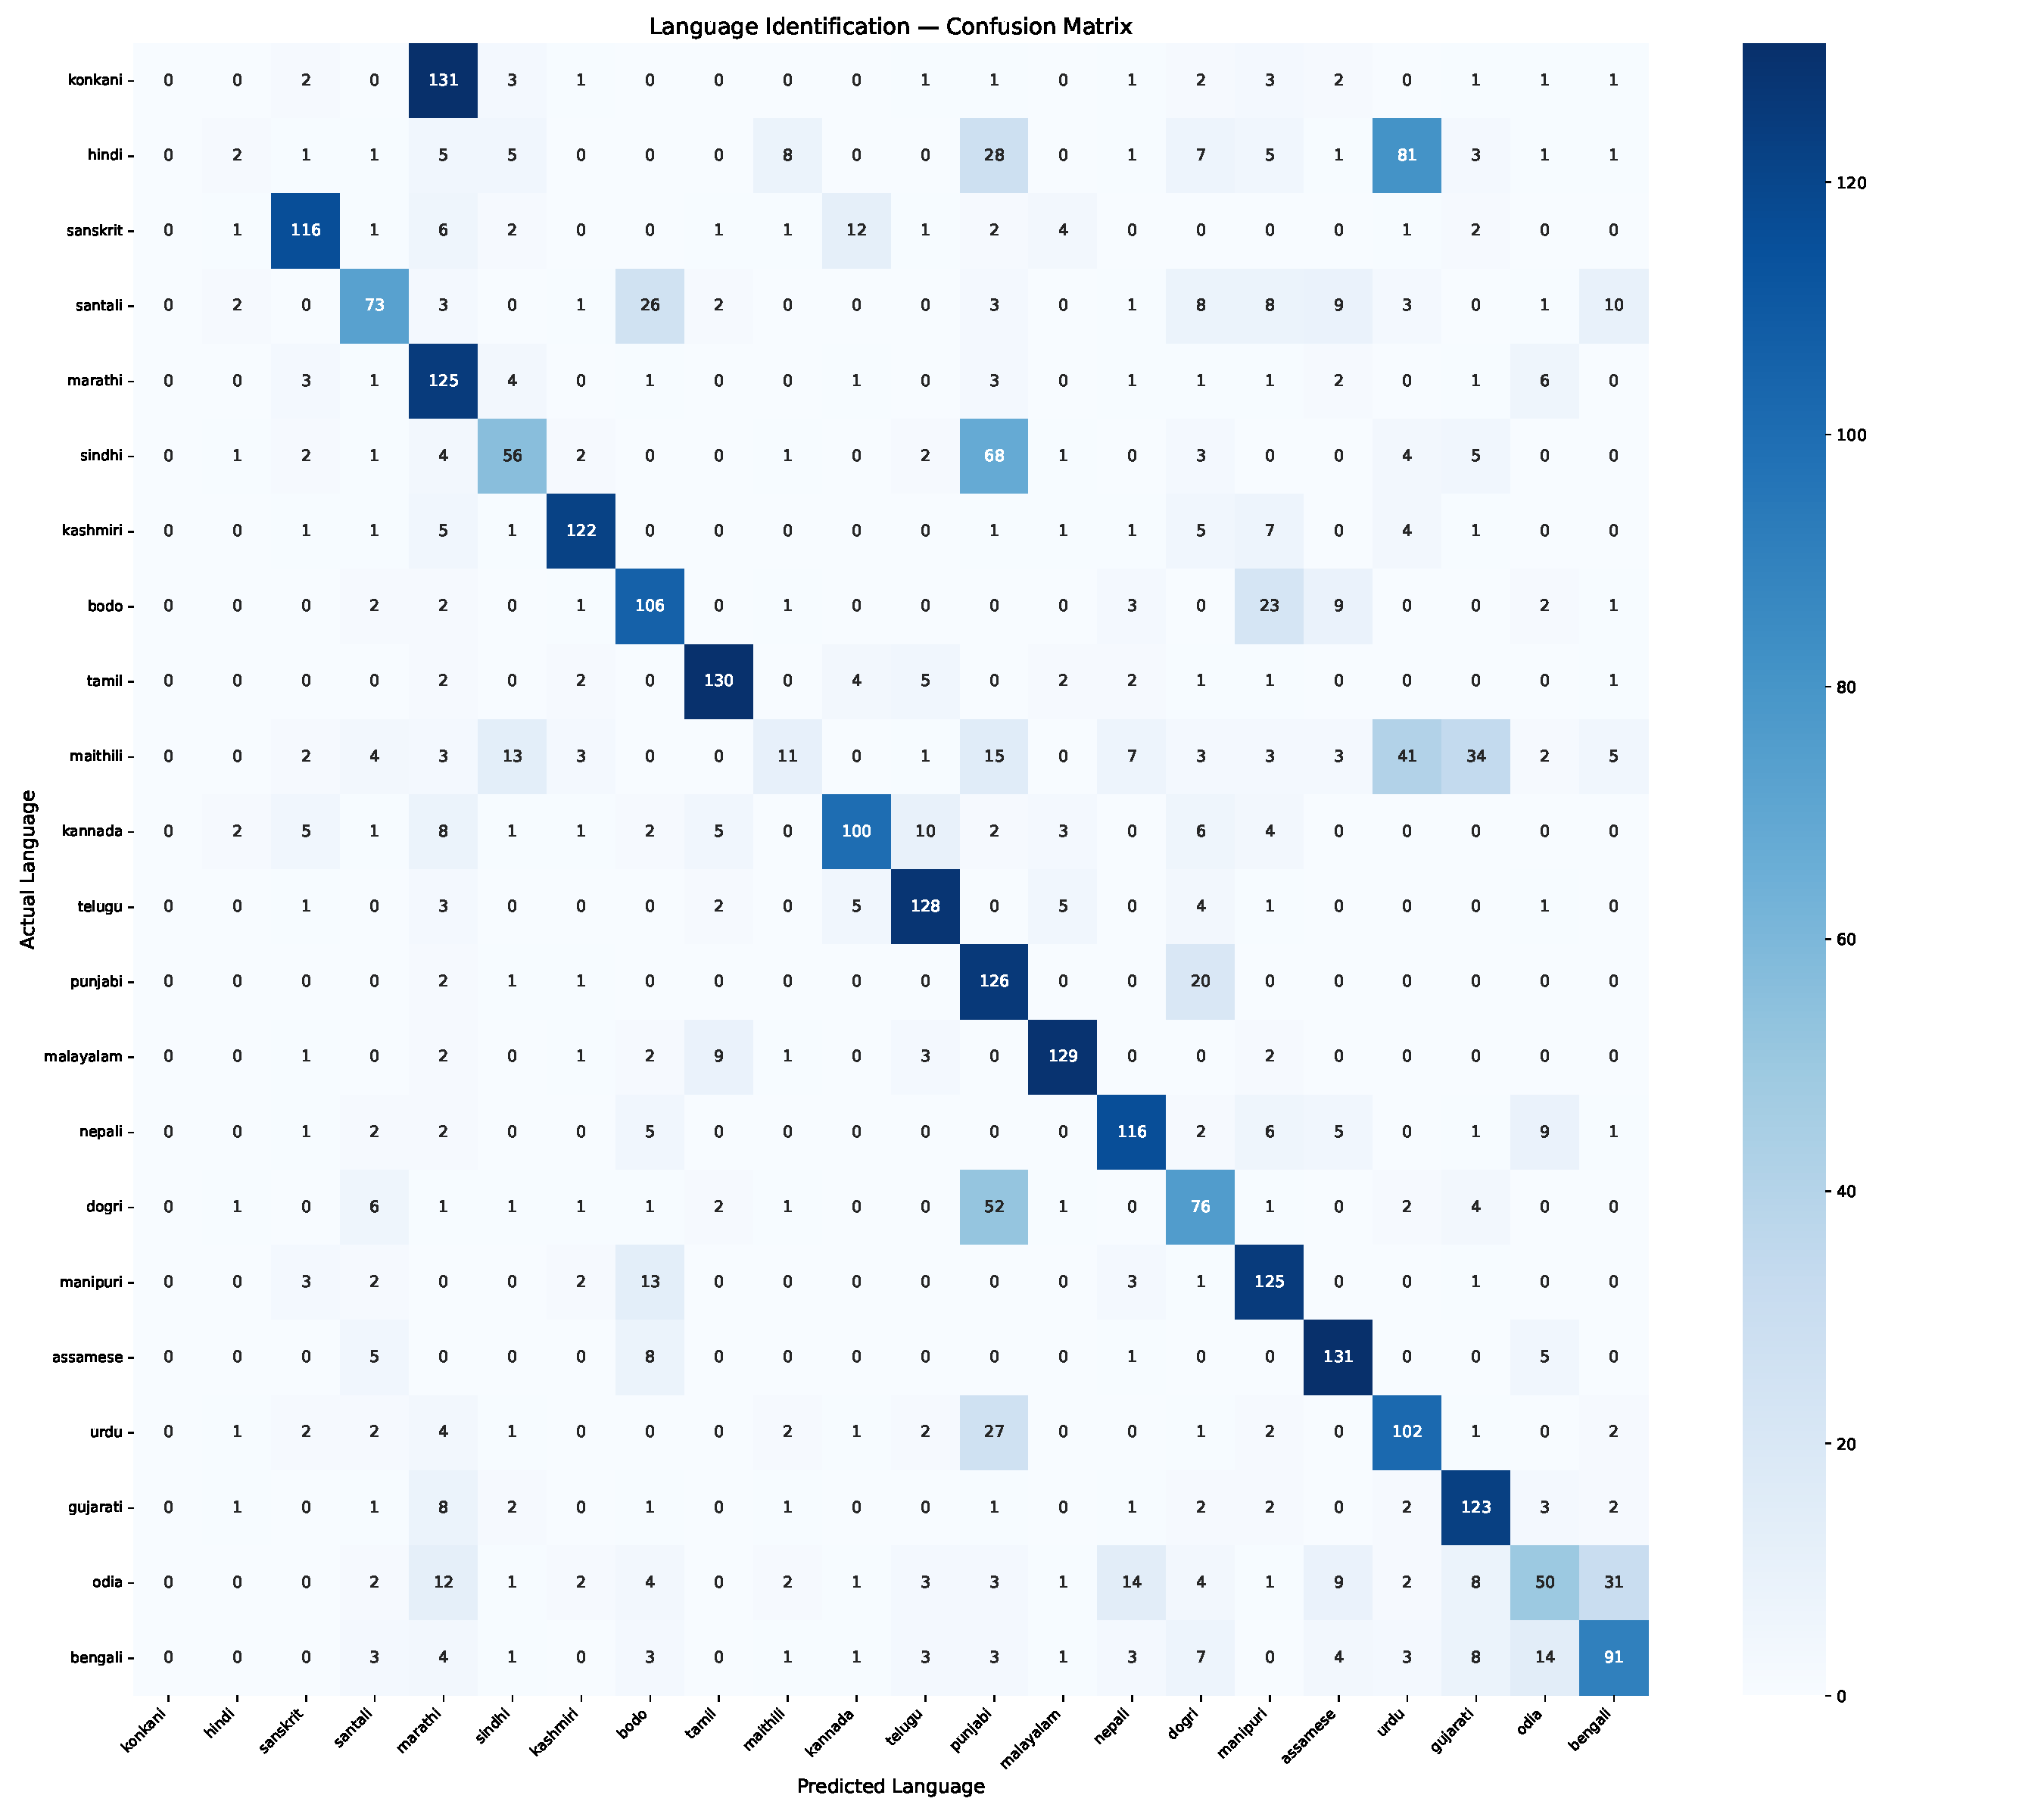
\includegraphics[width=1.0\columnwidth]{figures/figures_141033/confusion_matrix.pdf}
\caption{Confusion matrix (static augmentation) }
\label{fig:confusion_static_aug}
\end{figure}
\newpage

\begin{figure}[H]
\centering

\includegraphics[width=1.0\columnwidth]{figures/figures_baseline/tsne_language.png}
\caption{t-SNE visualization of embeddings - colored by language (baseline)}
\label{fig:tsne_lang_baseline}
\end{figure}


\begin{figure}[H]
\centering
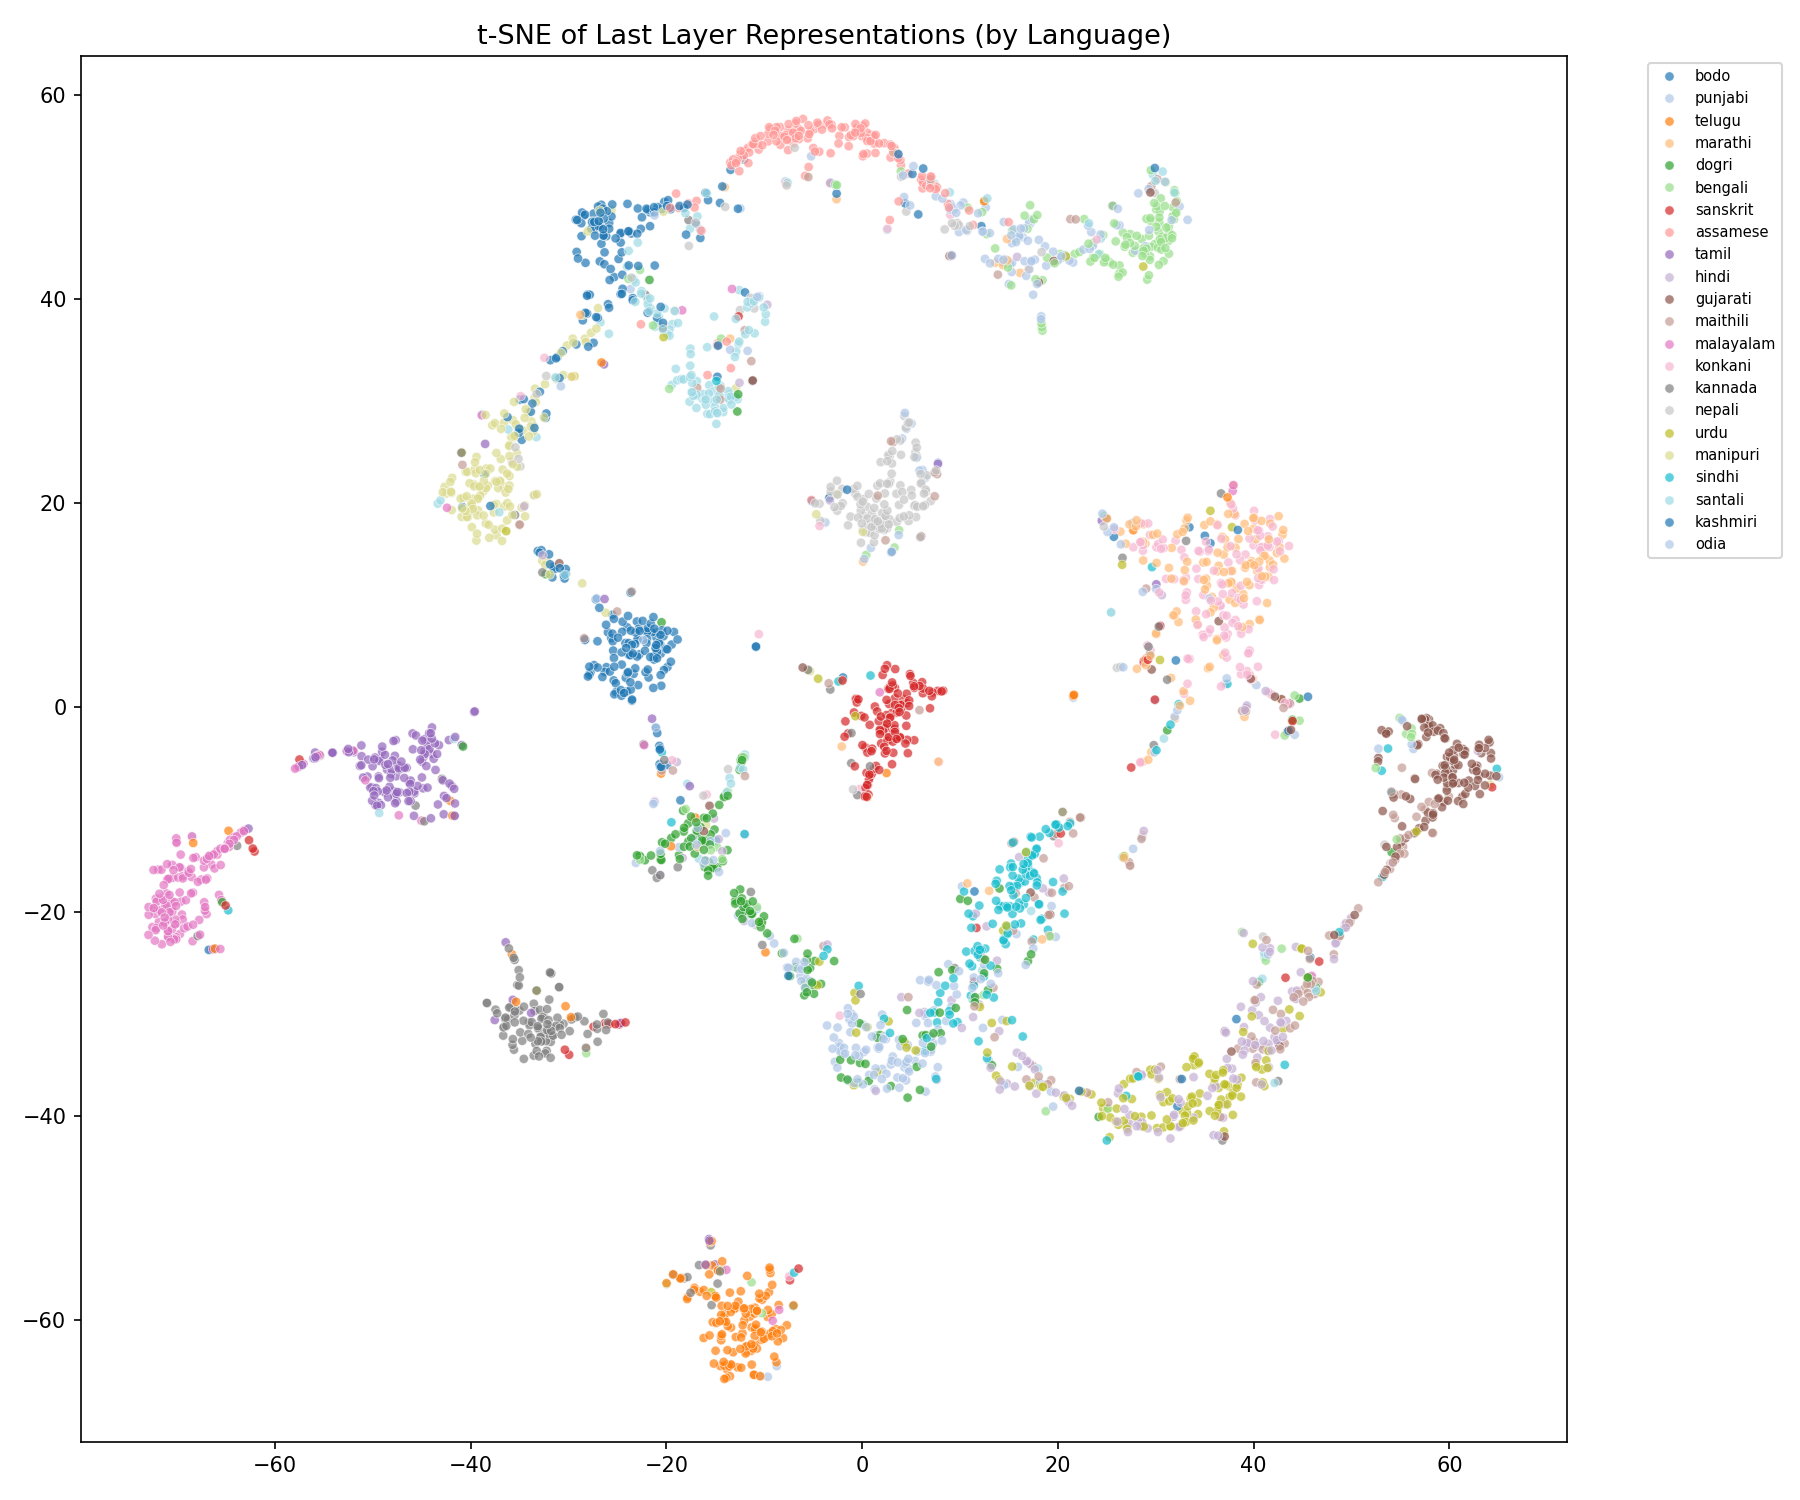
\includegraphics[width=1.0\columnwidth]{figures/figures_141033/tsne_language.png}
\caption{t-SNE visualization of embeddings - colored by language (static aug)}
\label{fig:tsne_lang_static}
\end{figure}


\begin{figure}[H]
\centering

\includegraphics[width=1.0\columnwidth]{figures/figures_baseline/tsne_speaker.png}
\caption{t-SNE visualization of embeddings - colored by speaker (baseline)}
\label{fig:tsne_spk_baseline}
\end{figure}


\begin{figure}[H]
\centering
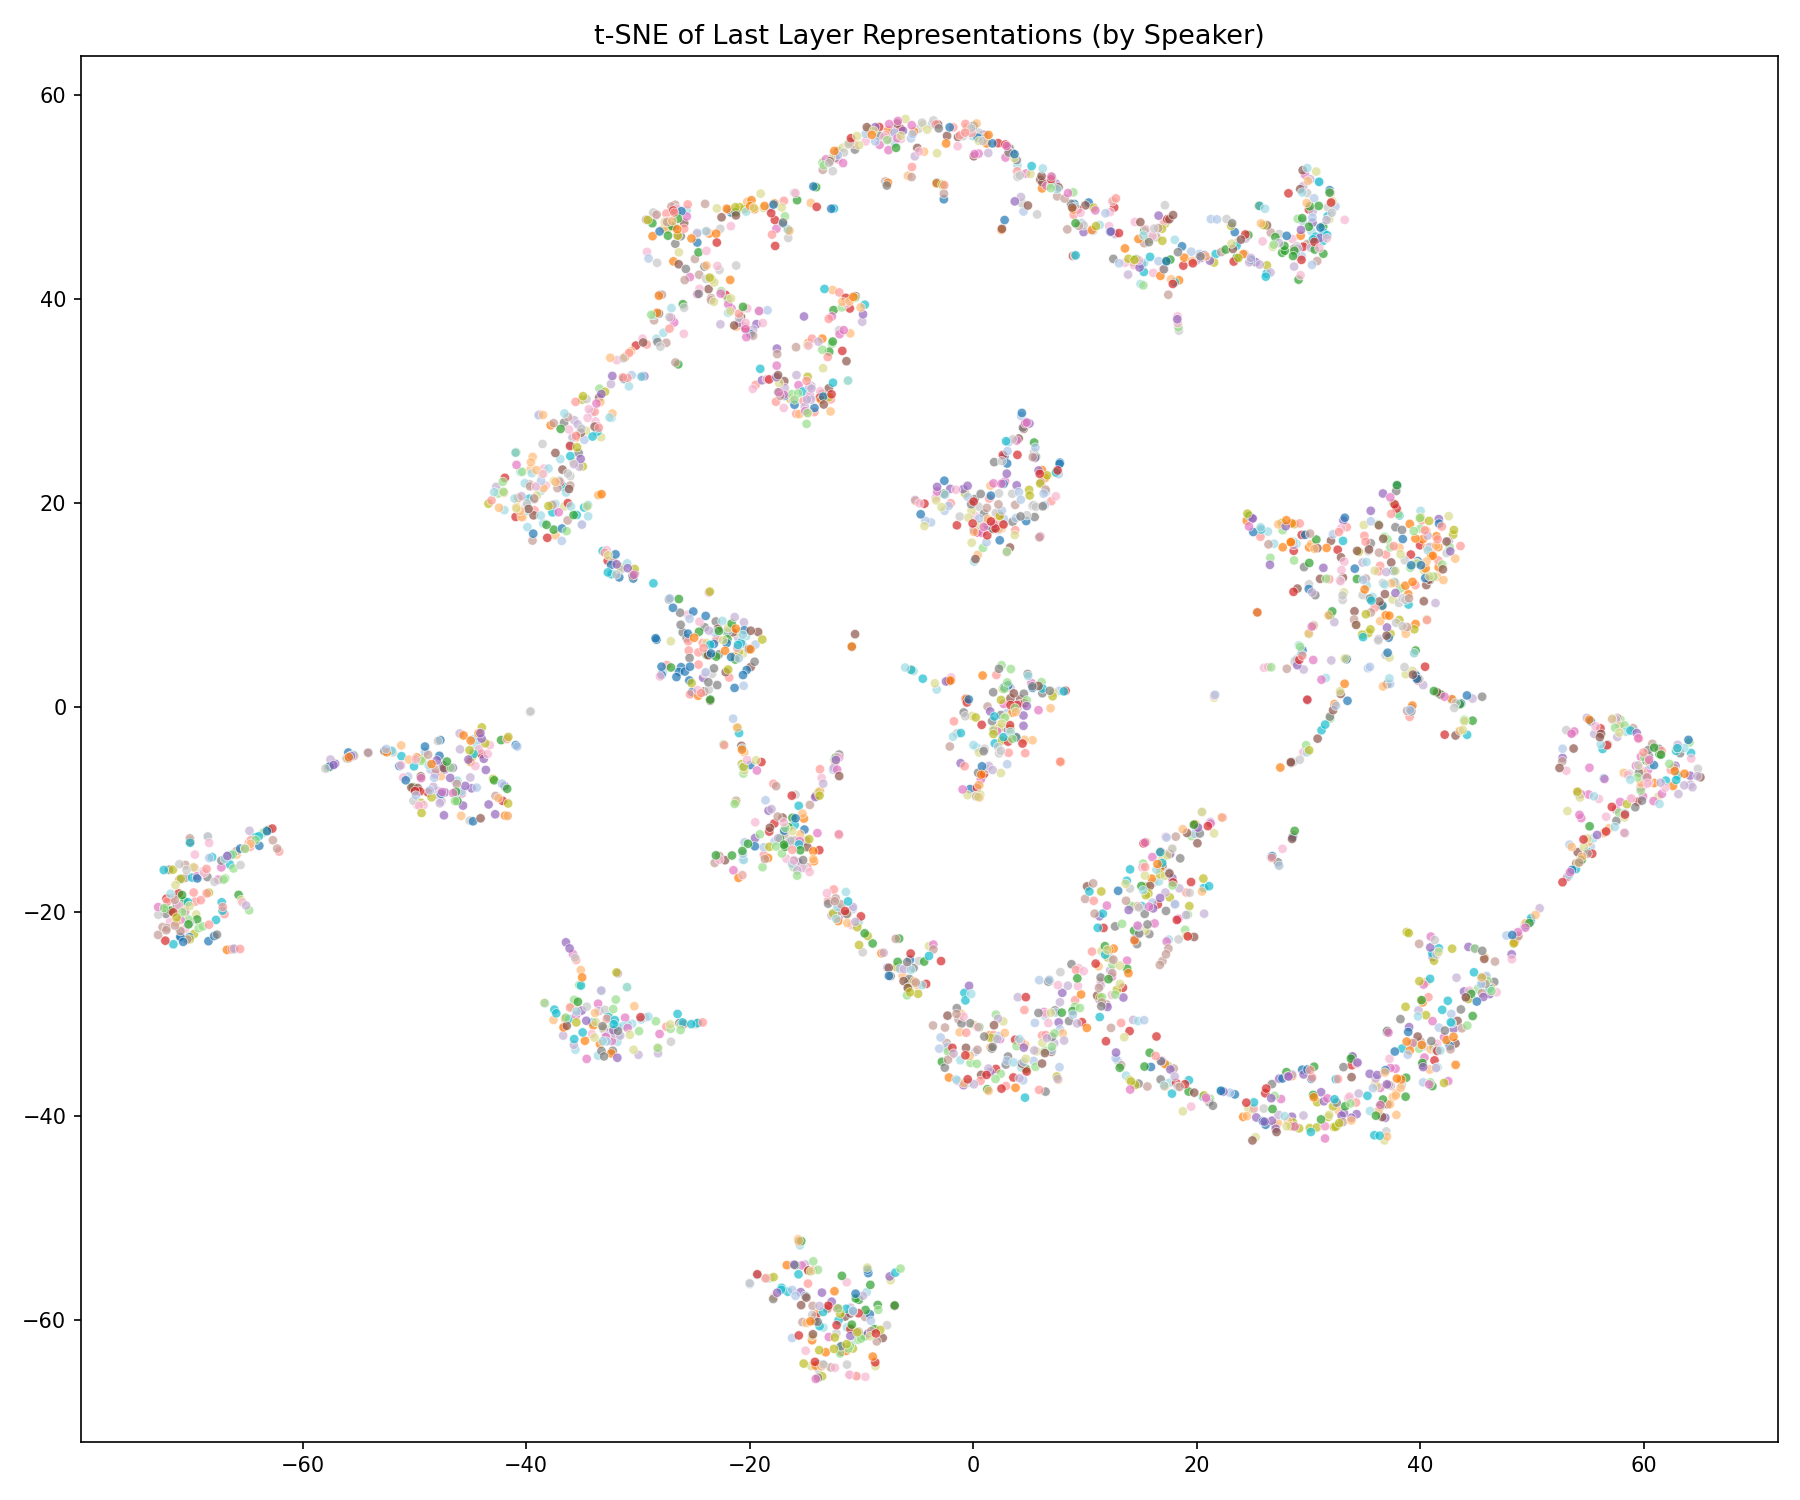
\includegraphics[width=1.0\columnwidth]{figures/figures_141033/tsne_speaker.png}
\caption{t-SNE visualization of embeddings - colored by speaker (static aug)}
\label{fig:tsne_spk_static}
\end{figure}



\end{document}
